\documentclass[a4paper]{jsarticle}
\usepackage[all]{xy}
\usepackage[dvipdfmx]{graphicx}
\usepackage{mathtools}
\usepackage{../math_note, exercise, enumitem}
\renewcommand{\thesection}{Ex7.\arabic{section}}

\newcommand{\coverU}{\mathfrak{U}}
\newcommand{\coverV}{\mathfrak{V}}

\newcommand{\Div}{\operatorname{Div}}
\newcommand{\Cl}{\operatorname{Cl}}
\newcommand{\CaCl}{\operatorname{CaCl}}
\newcommand{\nullCaCl}{\operatorname{CaCl}^{0}}
\newcommand{\Pic}{\operatorname{Pic}}

\begin{document}
    以下での($*$)とは,次のもの:
    \begin{itemize}
        \item integral,
        \item separated,
        \item noetherian, and
        \item regular in codimention one.
    \end{itemize}

    また,($\dagger$)は次のもの:
    $X$ :: noetherian scheme, 
    $\shS$ :: graded $\shO_X$-algebra
    となっている.
    また,$d \in \Z, d \geq 0$について,
    $\shS_d$ :: homogeneous part of $\shS$を$U \mapsto \shS(U)_d$.
    $X,\shS$は次をすべて満たす.
    \begin{itemize}
        \item $\shS$ :: quasi-coherent.
        \item $\shS=\bigoplus_{d \geq 0} \shS_d$.
        \item $\shS_0=\shO_X$.
        \item $\shS_1$ :: coherent $\shO_X$-module.
        \item $\shS$ :: locally generated by $\shS_1$ as $\shO_X$-algebra.
    \end{itemize}

\section{Surjective Mophism between Invertible Sheaves is Isomorphic.} %% Ex7.1 
    $X$ :: locally ringed space,
    $\shL, \shM$ :: invertible sheaves on $X$,
    $f: \shL \to \shM$ :: surjective mophism,
    とする.
    
    \paragraph{Proof 1.}
    任意の点$x \in X$をとり,$A=\shO_{X,x}$とおく.
    $f_x: \shL_x \to \shM_x$は同型写像を合成することで
    $\phi: A \to A$ :: surjective $A$-morphismと同一視出来る.
    $\phi$ :: surjectiveより,
    $\phi(\alpha)=1 \in A$となる$\alpha \in A$がとれる.
    また$\phi$は$A$-module morphismだから,$\alpha \phi(1)=1$.
    そこで$\psi: A \to A$を$a \mapsto \alpha a$と定義すれば,
    これが$\phi$の逆写像になる.
    よって$\phi, f_x$は同型.
    Prop1.1から,$f$ :: iso.

    \paragraph{Proof 2.}
    Matsumura, Thm2.4から分かる.
    これはNAK (or Nakayama's Lemma)からの帰結である.

    \begin{Remark}
        $k(x)$ :: residue fieldと
        $f_x: \shL_x \to \shM_x$をテンソルすると,
        $f_x \otimes \id{k(x)}$ :: surjective $k(x)$-module morphismが得られる.
        よって$\ker (f_x \otimes \id{k(x)})=0$.
        しかし,ここからNAKをつかって$\ker f_x=0$を導くことは出来ない.
        $k(x)$がflat $\shO_{X,x}$-moduleでなく,
        したがって$\ker (f_x \otimes \id{k(x)})$と$(\ker f_x) \otimes k(x)$の間に同型があることが
        言えないからである.
        このことはflat $\implies$ torsion-freeに気をつければすぐに分かる.
        同様の議論が$f_x$ :: injective(と$\coker f_x$)の場合に出来ることにも気づくが,
        このときは$\Z_2 \to \Z_2; 1 \mapsto 3$という反例がある.
    \end{Remark}

\section{Two Sets of Global Generators and Corresponding Morphisms.} %% Ex7.2 
    $k$ :: field,
    $X$ :: scheme /$k$,
    $\shL$ :: invertible sheaf on $X$,
    $S=\{s_0,\dots,s_m\}, T=\{t_0,\dots,t_n\}$ :: global generators of $\shL$.
    とする.
    ここで$S,T$は
    同じ線形(部分)空間$V \subseteq \Gamma(X, \shL)$を張るとする.
    また$n \leq m, d=\dim_k V$とする.

    $S,T$からそれぞれThm7.1のように定まるmorphismを$\phi_S, \phi_T$とする.
    $\phi_S$が次のように分解できることを示す.
    \[
        \xymatrix
        {
            X \ar@/_20pt/[rrrr]_-{\phi_S}\ar[r]^-{\phi_T}&
                \im \phi_T \ar@{^{(}->}[r]& \proj^m-L \ar[r]^-{\pi}&
                    \proj^n \ar[r]^-{\alpha}& \proj^n
        }
    \]
    ここで$\pi, \alpha$はそれぞれlinear projectionとautomorphismである.

    $X \to \proj^n$のmorphismを考えることは,
    $k[y_0,\dots, y_n]$の元$y_0,\dots,_n$の変換を考えることと同じである.
    これはThm7.1の証明を観察すれば分かる.
    二つの$k$-linear mapは$\phi_S^*, \phi_T^*$はそれぞれ,
    $y_i \mapsto s_i (i=0,\dots,n)$,
    $y_i \mapsto t_i (i=0,\dots,m)$で定まっている.
    したがって問題は,
    $t_0,\dots,t_m$を$s_0,\dots,s_n$へ
    変換するprojectionとautomorphismをつくる問題,
    と言い換えられる.

    今,次のような$(m+1) \times (n+1)$行列$Q$が存在する.
    \[
        \tatev{ s_0 \\ \vdots \\ s_n }
        =Q \tatev{ t_0 \\ \vdots \\ t_m }.
    \]
    $S,T$が$V$の生成系であることから$\rank Q=\dim V=:d$.
    $Q$は基本行列をいくつもかける(あるいは基本変形を繰り返し行う)ことにより,
    次の形に分解できる.
    \[
        Q=L P_{d} R~~
        \mwhere~ L \in PGL(m,k), R \in PGL(n,k)
    \]
    ただし行列$P_r ~(r=1,\dots,n+1)$は$r \times r$-identity matrix $I_r$をもちいて
    $P_{r}=
    \begin{bmatrix}
        I_r & 0 \\
        0 & 0
    \end{bmatrix}$
    と定義される行列である.
    (TODO: $P_{d}$を$P_{n+1}$に交換しても問題ない?)
    $L, P_{n+1}, R$が誘導するmorphismをそれぞれ$\beta, \tilde{\pi} ,\alpha$とすれば,
    $\alpha, \beta$はautomorphismであり,
    $\tilde{\pi}$はprojectionである.
    \[
        \xymatrix
        {
            \proj^m \ar[r]^-{\beta}& \proj^m
            \ar@{^{(}->}[r]^-{i}& \proj^m-L
            \ar[r]^-{\tilde{\pi}}& \proj^n
            \ar[r]^-{\alpha}& \proj^n
        }
    \]
    求める射はこの$\alpha$と,$\pi=\beta \circ i \circ \tilde{\pi}$である.
    また,$L=\zerosp(y_0,\dots,y_n) \subseteq \proj^m$の次元は$m-(n+1)$である.

\section{Morphism of $\proj^n \to \proj^m$ can be Decomposed into Common Ones.} %% Ex7.3
    $\phi: \proj^n_k \to \proj^m_k$を考える.
    $\shO_{\proj^m}(1), \shO_{\proj^n}(1)$
     :: invertible sheaves
    のglobal generatorをそれぞれ
    $\{x_0,\dots,x_m\}, \{y_0,\dots,y_n\}$
    とする.

    \subsection{$\im \phi=pt$ or $m \geq n$ and $\dim \im \phi=n$.}
%    $\eta: \Gamma(\proj^m, \shO_{\proj^m}(1)) \to \Gamma(\proj^m, \phi^* \phi_* (\shO_{\proj^m}(1)))$を
%    adjoint pair $\phi^* \dashv \phi_*$のunitから得られる射とする.
%    これが本文中で$\phi^*$と表記されているものである
    $s_i=\phi^*(x_i)~(i=0,\dots,m)$とおくと,
    $s_0,\dots,s_m$は$\shL:=\phi^*(\shO_{\proj^m}(1))$のglobal generatorである.
    $\shL$は$\proj^n$上のinvertible sheafだから,
    Cor6.17より,$\shL \iso \shO_{\proj^n}(d)$となる$d \in \Z$が存在する.
    Example7.8.3同様,$\shO_{\proj^n}(d)$は$|d|$次斉次単項式で生成される.

    \paragraph{$m<n \implies \dim \im \phi=0$.}
    \paragraph{$m \geq n \implies \dim \im \phi=n$.}

\section{If $X$ Admits an Ample Invertible Sheaf, then $X$ is Separated.} %% Ex7.4
    \subsection{Assumption of Thm7.6 $\implies$ $X$ :: separated.}
    $A$ :: noetherian ring,
    $X$ :: scheme of finite type /$A$とする.
    $\shL$ :: ample invertible sheaf on $X$が存在したとする.
    Thm7.6から,immersion $i: X \to \proj^n_A ~(n>0)$が存在する.
    これは$X$から$\proj^n_A$のlocally closed subschemeへのisomorphismである.
    これにprojection $\pr: \proj^n_A=\proj^n_{\Z} \times_{\Z} \Spec A \to \Spec A$を
    合成したものは,quasi-projective.
    \[\xymatrix
    {
        X \ar[r]^-{\sim}& U ~\ar@{^{(}->}[r]& Z ~\ar@{^{(}->}[r]& \proj^n_A \ar[r]^-{\pr}& \Spec A
    }\]
    $Z$は$\proj^n_A$のclosed subscheme,
    $U$は$Z$のopen subschemeである.
    $A,X$についての仮定から$\Spec A, X$ :: noetherian schemeがわかる
    \footnote
    {
        $f: X \to \Spec A$がfinite typeならば
        $f^{-1}\Spec A=X$はfinite affine open coverをもち,
        各affine open coverはfinitely generated $A$-algebraの$\Spec$である.
        finitely generated $A$-algebraは$A$からnoetherianを受け継ぐから,
        $X$ :: noetherian.
    }
    から,
    Thm4.9より,この射$X \to \Spec A$はseparated.
    
    \subsection{There is No Ample Invertible Sheaf on 
        \protect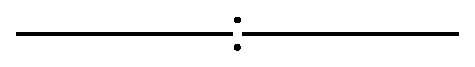
\includegraphics[width=2.5cm]{./images/affine_with_doubled_origin.eps} / a field $k$.}
    $k$ :: field,
    $X$ :: affine with doubled origin /$k$とする.
    より詳細に,$X$は$X_1=\Spec k[x_1], X_2=\Spec k[x_2]$を
    $U_1=X_1-\{O_1\}, U_2=X_2-\{O_2\}$で貼りあわせたものとする.
    ただし$O_1 \in X_1,O_2 \in X_2$は原点である.
    $X_i, U_i, O_i ~~(i=1,2)$はすべて$X$の部分集合とみなす.
    また$U=X_1 \cap X_2=X-\{O_1, O_2\}$とする.
    明らかに$U=U_1=U_2 \iso \affine^1-\{0\}=\Spec k[x_1, x_1^{-1}]$.
    また$x_1|_U=x_2|_U$.

    \paragraph{Plot.}
    まず,$X$上のinvertible sheaf全体$\Pic X$がどのようなものか調べる.
    これは$\Pic X \iso \Z$となる.
    $n \in \Z$に対応する$\Pic X$の元を$\shL_n$とする.
    次に,generated by global sectionであるようなinvertible sheafを考える.
    これは$\shL_0(=\shO_X)$しかない.
    すると任意の$m>0, n \neq 0$について
    \begin{align*}
        \shL_0 \otimes (\shL_n)^{\otimes m} &= \shL_{mn} \neq \shL_0. \\
        \shL_n \otimes (\shL_0)^{\otimes m} &= \shL_n \hspace{7pt}\neq \shL_0.
    \end{align*}
    なので,どのinvertible sheafもampleでない.

    \paragraph{$X$ :: noetherian integral scheme.}
    $X_1, X_2 \iso \affine^1=\Spec k[x_1]$とreducedがlocalな性質であることから
    $X$ :: noetherian reduced scheme.
    $X$ :: irreducibleも明らかだから,
    $X$ :: noetherian integral scheme.

    \paragraph{$\Pic X \ni \shL=\shL(D)$.}
    $\shL \in \Pic X$を任意にとる.
    $X$ :: integralとProp6.15より,
    $\shL=\shL(D)$となる$D \in \CaCl X$が存在する.
    Prop6.13の証明から$D$がどのような形のものか考えよう.
    Example 6.3.1, Cor 6.16より,$\Pic X_1, \Pic X_2$.
    なので$\shL|_{X_1} \iso \shO_{X_1}, \shL|_{X_2} \iso \shO_{X_1}$となる.
    Prop6.13の証明から,$D$は次のような形をしている.
    \[
        D=\{ \sect{X_1}{f_1}, \sect{X_2}{f_2} \}
        \mwhere
        f_1 \in \Gamma(X_1, \shK_{X_1}^*)=(k(x_1))^*,
        f_2 \in \Gamma(X_2, \shK_{X_2}^*)=(k(x_2))^*.
    \]

    \paragraph{$D \sim \{ \sect{X_1}{x_1^n}, \sect{X_2}{1} \}$.}
    Cartier divisorの定義から,
    $U=X_1 \cap X_2$において$f_1/f_2 \in \Gamma(U, \shO_U^*)$となっている.
    $U \subseteq X_1=\Spec k[x_1]$と考えると,
    $U=\Spec k[x_1]_{x_1}=\Spec k[x_1, x_1^{-1}]$.
    ($U \subseteq X_1$と見れば$U=\Spec k[x_2,x_2^{-1}]$であるが,どちらでも同じである.)
    そして
    \[ \Gamma(U, \shO_U^*)=(k[x_1, x_1^{-1}])^*=\{ \alpha x_1^{n} \mid \alpha \in k^*, n \in \Z \}. \]
    であるから,$f_1/f_2=\alpha x_1^{n} (\iff f_2/f_1=(\alpha x_2^n)^{-1})$と書ける.
    よって
    \[
        D
        =\{ \sect{X_1}{\alpha x_1^n f_2}, \sect{X_2}{f_2} \}
        \mwhere
        f_2 \in \Gamma(X_2, \shK_{X_2}^*)=(k(x_2))^*.
    \]
    再び$X$ :: integralから,$\shK_X$はconstant sheafであり,
    したがって$f_2 \in K=\Gamma(X, \shK_X^*)$となる.
    なので
    $\{ \sect{X_1}{f_2}, \sect{X_2}{f_2} \}$はprincipal.
    加えて$\{ \sect{X_1}{\alpha}, \sect{X_2}{1} \} \in \Gamma(X, \shO_X^*)$なので
    \footnote
    {
        ここの部分はProp6.13cを用いて
        \[
            \shL(\{ \sect{X_1}{\alpha}, \sect{X_2}{1} \})
            =\shO_X
            =\shL(\{ \sect{X_1}{1}, \sect{X_2}{1} \})
        \]
        故に
        $\{ \sect{X_1}{\alpha}, \sect{X_2}{1} \}
            =\{ \sect{X_1}{1}, \sect{X_2}{1} \}$,
        と理解しても良い.

    },
    結局$D \sim \{ \sect{X_1}{x_1^n}, \sect{X_2}{1} \}$.

    \paragraph{$\Pic X \iso \Z$.}
    $n \in \Z$に対し,次のように定める.
    \[ D_n=\{ \sect{X_1}{x_1^n}, \sect{X_2}{1} \},~~~ \shL_n=\shL(D_n). \]
    これは次の写像を定める.
    \begin{defmap}
        {}& \Z& \to& \CaCl X \\
        {}& n& \mapsto& D_n
    \end{defmap}
    明らかに$D_m+D_n=D_{m+n}, \shL_m \otimes \shL_n=\shL_{m+n}$だから,
    これは加法群としての全射準同型.
    最後に,単射であることを見よう.
    $D_n=D_0$ならば,
    \[ D_n=\{ \sect{X_1}{x_1^n}, \sect{X_2}{1} \}=\{ \sect{X_1}{1}, \sect{X_2}{1} \}=D_0. \]
    なのでsectionの同値の定義から$x_1^n/1 \in \Gamma(X_1, \shO_{X}^*)=k^*$.
    これは$n=0$を意味している.

    \paragraph{Globally Generated Invertible Sheaf on $X$.}
    $n \in \Z$を任意にとり,
    $\{g_i\}_i \subseteq \Gamma(X, \shL_n)$が$\shL_n$のglobal generatorsであるとしよう.
    $\shL_n=\shL(D_n)$だから,
    $\shL_n|_{X_1}$は$x_1^n$でgenerateされ,
    $\shL_n|_{X_2}$は$1$でgenerateされている.
    特に後者から,$\shL_n|_{U}$は$1$でgenerateされている.
    したがってstalkで見れば,次のようになっている.
    \begin{align*}
        \Forall{P \in X_2}
        &\langle (g_i)_{P} \rangle_i
            \hspace{3.5pt}
            =(\shL_n)_{P}
            \hspace{3.7pt}
                =\shO_{X, P}
                    &&\text{  as  $\shO_{X, P}$-module.} \\
        &\langle (g_i)_{O_1} \rangle_i
            =(\shL_n)_{O_1}
                =(x_1^n)_{O_1} \shO_{X, O_1}
                    &&\text{  as  $\shO_{X, O_1}$-module.}
    \end{align*}
    これらを可換環に翻訳し,
    $g_i$を$g_i|_{X_2}, g_i|_U, g_i|_{X_1}$の順に求めていく.
    $X_2=\Spec k[x_2]$だから,
    $P$に対応する素イデアル$\I{p} \subset k[x_2]$がとれる.
    また,$g_i|_{X_2} \in \Gamma(X_2, \shO_X)=k[x_2]$.
    $\shO_{X,P}=\shO_{X_2, P}=k[x_2]_{\I{p}}$であり,
    したがって$k[x_2]_{\I{p}}$-moduleとして
    $\langle (g_i|_{X_1})_{\I{p}} \rangle=k[x_2]_{\I{p}}$.
    なので,次が成り立つ.
    \[
        \Forall{\I{p} \in \Spec k[x_2]} \Forall{i}
        (g_i|_{X_2})_{\I{p}} \in (k[x_2]_{\I{p}})^*=k[x_2] \setminus \I{p}.
    \]
    よって$g_i|_{X_2} \in (k[x_2])^*=k^*$がわかる.
    特に$g_i|_{U}=\alpha \in k^*$と書ける.
    変形して,$(g_i|_{X_1}-\alpha)|_U=0$.
    ($\alpha \in \Gamma(X_1, \shO_{X}^*)$とみなしている.)
    $U=D(x_1) \subset \Spec k[x_1]=X_1$なので,
    Lemma5.3より,十分大きな$r>0$について$x_1^r(g_i|_{X_1}-\alpha)=0$ on $X_1$.
    しかし$\Gamma(X_1, \shO_{X})=k[x_1]$はdomainなので
    結局$g_i|_{X_1}=\alpha$ on $X_1$.
    $\langle (g_i)_{O_1} \rangle_i=(x_1^n)_{O_1} \shO_{X, O_1}$
    と合わせて$g_i|_{X_1}=x_1^{n} \in k^*$が得られ,$n=0$となる.
    以上より,$\shL_0$のみがgenerated by global sectionsである.

    \paragraph{Another Proof: Globally Generated Invertible Sheaf on $X$.}
    $n \in \Z$をとり,
    $\{g_i\}_i \in \Gamma(X, \shL_n)$を$\shL_n$のglobal generatorとする.
    localには$\shL_n$のgeneratorは$x_1^n, 1$で与えられており,
    $\{g_i\}_i$達もlocalには$x_1^n, 1$と一致している.
    \begin{align*}
        \{ g_i|_{X_1}\}_i=\{ x_1^n, 1\} \subset \Gamma(X_1, \shK_{X_1}^*/\shO_{X_1}^*),
        &&&
        \{g_i|_{X_2}\}_i=\{1\} \subset \Gamma(X_2, \shK_{X_2}^*/\shO_{X_2}^*)
    \end{align*}
    となる.
    右から$\{g_i|_{X_2}\}_i, \{g_i|_U\}_i \subseteq k^*$が直ちに得られる.
    なので前の証明と同様に$x_1^n \in k^*$が分かり,
    よって$n=0$.

    \paragraph{資料.}
    詰まったところでは次のページを参考にした:
    \url{ https://math.stackexchange.com/questions/70042 }.
          
\section{ Ample and Very Ample are Inherted by Tensor Products.} %% Ex7.5 
          
\section{The Riemann-Roch Problem.} %% Ex7.6 

\section{Some Rational Surfaces.} %% Ex7.7 

\section{Sections of $\pi: \P(\shE) \to X$
    $\leftrightarrow$ Quotient Invertible Sheaves of $\shE$.} %% Ex7.8 

\section{ } %% Ex7.9 

\section{$P^n$-Bundles Over a Scheme.} %% Ex7.10 

\section{Different Sheaves of Ideals can Give Rise to Isomorphic Blow Up Schemes.} %% Ex7.11 

\section{ } %% Ex7.12 

\section{* A Complete Nonprojective Variety.} %% Ex7.13 

\section{ } %% Ex7.14 


\end{document}
